\section{Przekształcenie otrzymanej odpowiedzi skokowej}

Uzyskaną odpowiedź procesu na zmianę sygnału sterującego z punktu pracy $Upp=\num{32.0}$ na $Umax=\num{55.0}$ przekształcono w następujący sposób:\newline
\indent - Ograniczono (przycięto) czas zmiany sterowania u oraz wyjścia y od chwili skoku do ustabilizowania,\newline
\indent - Wykres sterowania u przesunięty został o wartość początkową $Upp=\num{32.0}$ w dół,\newline
\indent - Wykres wyjścia y przesunięty został o wartość początkową $Ypp=\num{36.8}$ w dół,\newline
\indent - Wykres sterowania $u$ i wyjścia $y$ podzielono przez zmianę sterowania $\Delta u=\num{23.0}$.

Uzyskana odpowiedź skokowa daje nam wektor współczynników $s$,
który wykorzystywany będzie w algorytmie DMC.

\begin{figure}[H]
    \centering
    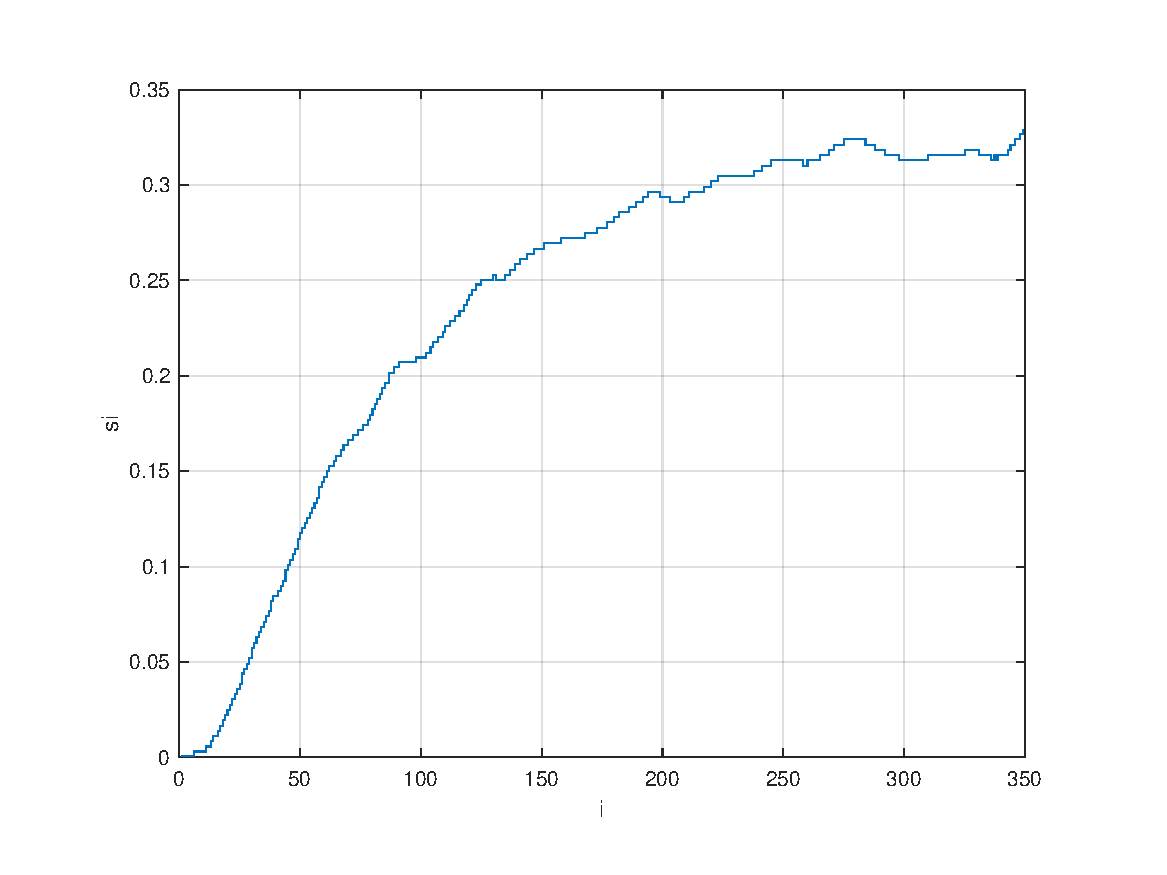
\includegraphics[scale=0.75]{../lab/zad_3/zad3s.pdf}
    \caption{Wykres współćzynników s}
\end{figure}

W ramach pierwszego laboratorium zespół miał za zadanie 
zaproksymować odpowiedź skokową pozyskaną ze stanowiska grzewczo-chłodzącego w celu 
późniejszego jej wykorzystania w algorytmie DMC. 
Aproksymacja została wykonana jako człon inercyjny drugiego rzędu z opóźnieniem. 
Opisany jest on następującą transmitancją: 

$$G(s)=\frac{K}{(sT_{1}+1)(sT_{2}+1)}e^{-T_{d}s}$$

Powyższa transmitancja po przekształceniu do dziedziny czasu dyskretnego i przejściu na postrać równania różnicowego:
%$$G(z)=\frac{z-1}{z}Z\Big[\frac{G(s)}{s})\Big]$$

$$y[k]=b_{1}u[k-T_{D}-1]+b_{2}u[k-T_{D}-2]+a_{1}y[k-1]+a_{2}y[k-2]$$
 
Na podstawie danych pozyskanych ze stanowiska laboratoryjnego dobrano parametry 
$T_{1}$, $T_{2}$, $K$, $T_{d}$, tak aby błąd dopasowania, 
rozumiany jako suma kwadratów kolejnych uchybów sterowania, był jak najmniejszy. 
Należy jednak pamiętać, że wielkość Td może przyjmować tylko wartości całkowite 
(ze względu na zastosowany czas dyskretny). 
W celu doboru parametrów modelu wykorzystano funkcję optymalizacyjną $fmincon$ programu MATLAB, 
jako parametr optymalizacji wybrano błąd dopasowania 
(rozumiany jako suma kwadratów błędów dla kolejnych elementów odpowiedzi skokowych), 
ponieważ im mniejszy błąd dopasowania tym lepsza aproksymacja. \newline
Otrzymane parametry aproksymacji to: \newline
\indent $$T_{1}=\num{7.59}
\indent T_{2}=\num{62.4}
\indent K=\num{0.32}
\indent T_{d}=\num{10.0}$$

\begin{figure}[H]
    \centering
    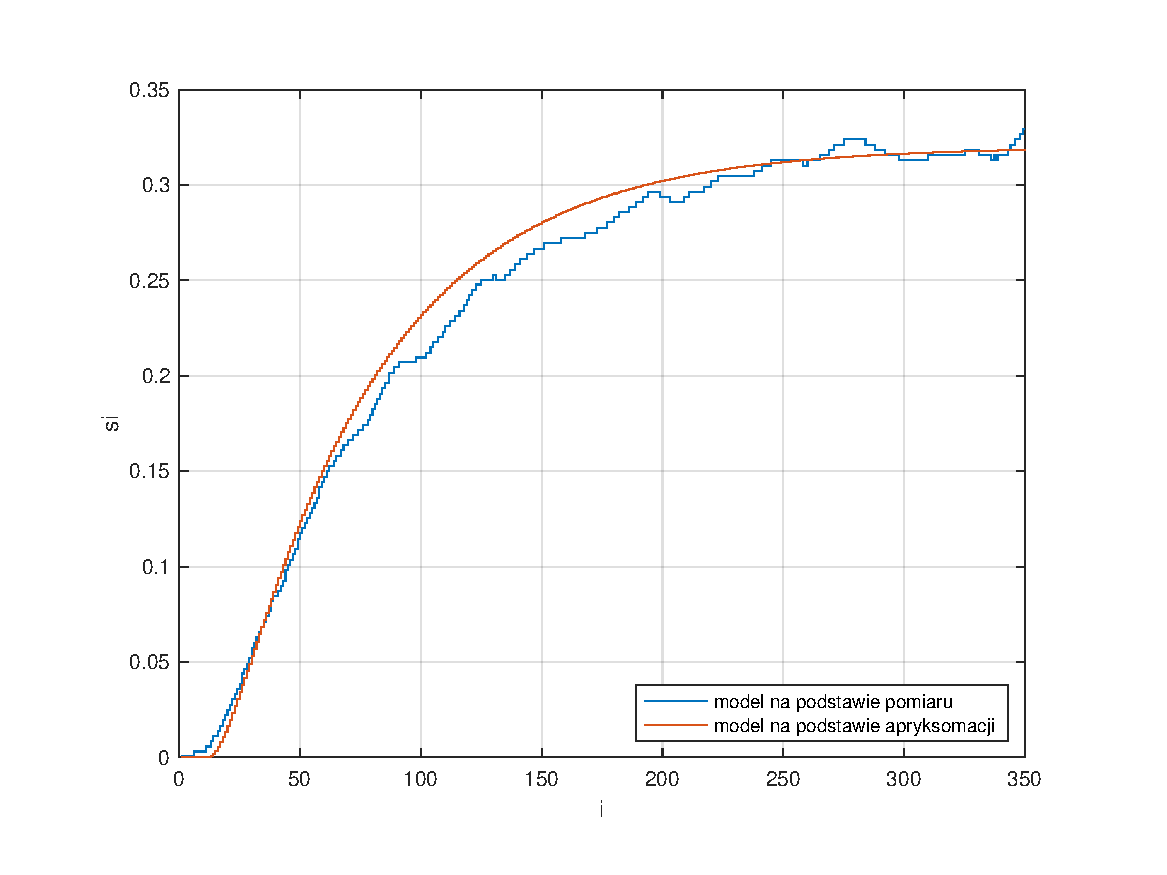
\includegraphics[scale=0.75]{../lab/zad_3/zad3aprox.pdf}
    \caption{Aproksymacja odpowiedzi skokowej}
\end{figure}

